\documentclass[10pt]{extarticle}

\usepackage[landscape,margin=0.25in]{geometry}
\usepackage{graphicx}

\begin{document}

\thispagestyle{empty}
\centering

\textit{Dwarves} \hfill \today

\begin{figure}[!ht]

  \includegraphics[width=10.5in]{player-1.png}
  \vskip 0.5em\hrule\vskip 1em
  \includegraphics[width=10.5in]{player-2.png}
  \vskip 0.5em\hrule\vskip 1em
  \includegraphics[width=10.5in]{player-3.png}
  \vskip 0.5em\hrule\vskip 1em
  \includegraphics[width=10.5in]{player-4.png}
  \vskip 0.5em\hrule\vskip 1em
  \includegraphics[width=10.5in]{player-5.png}
  \vskip 0.5em\hrule\vskip 1em 
  \includegraphics[width=10.5in]{player-6.png}
  \vskip 0.5em\hrule\vskip 1em
  \includegraphics[width=10.5in]{player-7.png}
\end{figure}

\begin{minipage}{0.48\textwidth}
  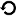
\includegraphics[width=0.15in]{resources/icons/refresh-16.png} loop sample (default)\\
  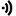
\includegraphics[width=0.15in]{resources/icons/rss-16.png} reverb, keep close to zero if not indicated, \texttt{??} means it's up to you \\
  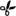
\includegraphics[width=0.15in]{resources/icons/cut-16.png} slice to whatever interests you, or just use the entire sound \\
  \texttt{\#x} playback rate, \texttt{??} means it's your choice \\
  % \phantom{\quad} volume is indicated by fill
\end{minipage}\hfill
\begin{minipage}{0.48\textwidth}
\end{minipage}

\end{document}
